%
% $Id: ch02_relatedwork
%
%   *******************************************************************
%   * SEE THE MAIN FILE "AllegThesis.tex" FOR MORE INFORMATION.       *
%   *******************************************************************
\chapter{Related Work}\label{ch:relatedwork}
In this chapter, we discuss the different algorithms we integrate with MCTS, as well as describe existing implementations of game-playing agents which use these techniques.  The chapter is organized by algorithm, with each section discussing a specific algorithm and existing implementation of the algorithm.  We discuss how each existing system has been implemented, and briefly overview how well these implementations have performed.

\section{Genetic Algorithms}
A Genetic Algorithm (GA) is an optimization or search algorithm based on Darwin's theory of evolution \cite{fuzzymitchell99}.  The algorithm borrows ideas from biology such as genes and chromosomes, as well as the concepts of crossover and mutation.  In biology, a gene can be thought of an encoding of a trait, such as eye color, while a chromosome is a collection of genes which make up the "blueprint" of an organism.  Crossover is the process of selecting genes from two parent chromosomes to create a child chromosome, while mutation is a random alteration of a gene.  Before explaining how a GA works, it is important to first understand what these terms, and a few others, mean in regards to the algorithm.

In GAs, a chromosome refers to a possible solution to a problem, which is often encoded as a string of bits.  The genes are the various chunks of the chromosome which encode a specific element of the solution.  For example, consider an agent from a GA which trades on the stock market.  Every stock indicator (such as change in price, volume, etc.) may be represented by a gene consisting of 4 bits --- the value of each gene determines how highly it considers that indicator compared to the others.  The agent's chromosome is made up of a collection of these genes and is its overall trading strategy.  Crossover might consist of randomly selecting genes from two agents to create a new chromosome, while mutation might be	having a possibility of flipping a random bit in a gene.

Furthermore, the entire collection of chromosomes (i.e. potential solutions) is referred to as the \textit{population}.  The \textit{fitness} of a particular chromosome is essentially how good of a solution it provides; the \textit{fitness formula} $f(x)$ is the method of calculating fitness.  On each iteration of the algorithm, a new population is created --- each population is referred to as a \textit{generation}.

A GA begins by generating a random population for the problem space.  Then, the fitness of each member of the population is calculated by some $f(x)$; a chromosome's fitness may also just be an amount relative to the fitness of other chromosomes.  Next, we repeat the following steps until $n$ new chromosomes have been created:
\begin{itemize}
\item Select a pair of chromosomes (parents) from the population.  The probability of selection is higher for chromosomes with a higher fitness;
\item Via some predetermined method, perform a crossover between the two parents to create a child chromosome;
\item Randomly mutate the child chromosome with a predetermined probability $p_m$.
\end{itemize}

Once $n$ children have been created, we replace the $n$ lowest performing children in the population with the new children --- this creates our new generation.  This process of evaluation, selection, crossover, and mutation repeats itself until either (a) a desired fitness is reached or (b) a certain number of generations has been produced.  Figure \ref{fig:GA} depicts the GA algorithm visually.

Note that the crossover portion of the algorithm helps improve the overall fitness of the population over time, while the mutation helps maintain diversity in the population and protect from the chromosomes becoming overfit.  These concepts, as well as the random distribution of chromosomes over the search space  at the start, help keep the algorithm from getting stuck at local maxima.

\begin{figure}[h]
    \centering
    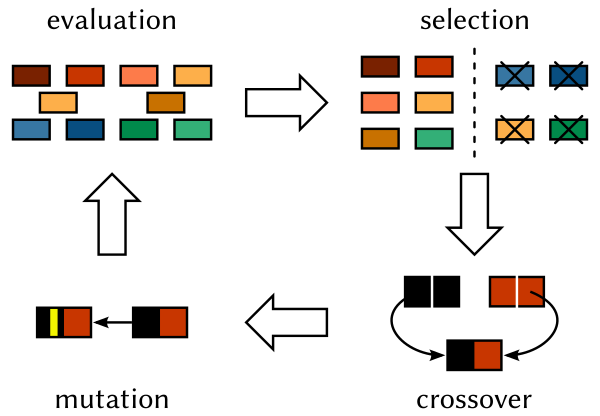
\includegraphics[clip, scale=.3]{images/GA1.png}
    \caption{Process of a Genetic Algorithm}
    \label{fig:GA}
\end{figure}

A GA can be integrated with MCTS to fine-tune both the tree policy and the default policy.  In \cite{Cazenave2007}, Cazenave created a Go-playing agent which utilized MCTS whose UCT formula was optimized by a genetic algorithm.  He compared three agents: one whose tree policy was a static UCT, one which used a tree policy known as RAVE, and finally one with UCT whose bias parameter he optimized with a GA.  The agent with the optimized bias parameter outperformed the other two.

More interesting is Lucas \etals fast evolution method \cite{lucas2014fast}.  Rather than pre-optimize the MCTS algorithm, Lucas \etal developed a system which optimizes its performance on the fly.  Rather than evaluate individuals after entire game playouts, each iteration of the MCTS algorithm is followed by the evaluation of a number of individuals all working on the same search tree.  At every iteration, both the tree policy and the default policy is biased towards the most fit individuals policy.  The results of Lucas \etals work were positive, showing their algorithm performed better than a standard MCTS agent in 99\% of runs in games called \textit{Space Invaders} and \textit{Mountain Car}.

\section{Artificial Neural Networks}
An Artificial Neural Network (ANN) is a machine learning method which, like genetic algorithms, has a basis in biology --- it is often viewed as a simplified model of how the brain solves problems \cite{aimodern}.  ANNs  are commonly used for pattern recognition or data classification.  Very abstractly speaking, an ANN is simply a cluster of nodes connected by links, with each link having a numerical weight associated with it.

More specifically, each node takes in a number of inputs and produces a decimal output (usually a number between 0 and 1).  Some nodes are connected to the network's environment and are called \textit{input nodes} or \textit{output nodes}.  As one might imagine, input nodes are those which receive data or information from the environment, and output nodes give us the a value based on the network's inputs.  Any other nodes in the network are called \textit{hidden nodes} because they cannot be directly observed/accessed from the environment --- their inputs are either the output of input nodes or other hidden nodes.

Each link between the nodes has a weight associated with it, which essentially just tells each node how much to ``value'' a given input.  There are a few ways in which the nodes and links of an ANN can be structured, and each type of structure (or \textit{topology}) results in different computational properties.  Here, we will specifically talk about \textit{feed-forward} networks as this is the structure we will be using in our experiments.  The other main type of network is the \textit{recurrent} ANN, and often has a more complex topology.

In a feed-forward network, links are unidirectional and there are no cycles --- a feed-forward network is a directed acyclic graph.  The network is organized in layers, with each node only linking to nodes in the next layer.  Although this structure is much simpler than that of a recurrent network, feed-forward networks have sufficient computational abilities for most pattern recognition and classification problems \cite{pruningsource7}.  A simple illustration of a feed-forward ANN with one hidden layer can be seen in Figure \ref{ref:simpleann}.

\begin{figure}[h]
\centering
\def\layersep{2.5cm}

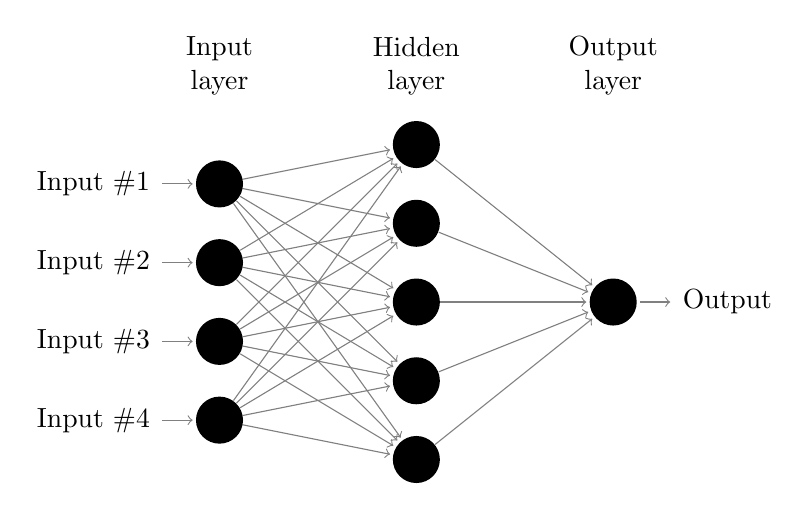
\begin{tikzpicture}[shorten >=1pt,->,draw=black!50, node distance=\layersep]
    \tikzstyle{every pin edge}=[<-,shorten <=1pt]
    \tikzstyle{neuron}=[circle,fill=black!25,minimum size=17pt,inner sep=0pt]
    \tikzstyle{input neuron}=[neuron, fill=black];
    \tikzstyle{output neuron}=[neuron, fill=black];
    \tikzstyle{hidden neuron}=[neuron, fill=black];
    \tikzstyle{annot} = [text width=4em, text centered]

    % Draw the input layer nodes
    \foreach \name / \y in {1,...,4}
    % This is the same as writing \foreach \name / \y in {1/1,2/2,3/3,4/4}
        \node[input neuron, pin=left:Input \#\y] (I-\name) at (0,-\y) {};

    % Draw the hidden layer nodes
    \foreach \name / \y in {1,...,5}
        \path[yshift=0.5cm]
            node[hidden neuron] (H-\name) at (\layersep,-\y cm) {};

    % Draw the output layer node
    \node[output neuron,pin={[pin edge={->}]right:Output}, right of=H-3] (O) {};

    % Connect every node in the input layer with every node in the
    % hidden layer.
    \foreach \source in {1,...,4}
        \foreach \dest in {1,...,5}
            \path (I-\source) edge (H-\dest);

    % Connect every node in the hidden layer with the output layer
    \foreach \source in {1,...,5}
        \path (H-\source) edge (O);

    % Annotate the layers
    \node[annot,above of=H-1, node distance=1cm] (hl) {Hidden layer};
    \node[annot,left of=hl] {Input layer};
    \node[annot,right of=hl] {Output layer};
\end{tikzpicture}
\caption{A simple feed forward ANN}
\label{ref:simpleann}
\end{figure}

With this network structure, learning is just the process of tuning the weights of the links to better fit the data in a training set.  For example, suppose we have a network which we are training to identify handwritten numbers.  If, during training, it identifies a number as a `2' when it is really a `3', it can make a very small adjustment in its weights to get a little closer to thinking it is a `3'.  Over a large data set, these small adjustments add up to create a rather well-generalized network.  Statistically speaking, the ANN is an abstracted, finely tuneable nonlinear regression of the training data \cite{aimodern}. 

In \cite{annpruning}, Burger \etal provide a method of integrating a feed-forward ANN with MCTS --- specifically, they integrate the ANN into the UCT tree policy.  The ANN is used to \textit{prune} the search tree as the agent searches.  That is, it determines that certain portions of the tree are undesirable and removes them from the search space.  Assuming this is done accurately, the tree policy becomes more efficient as it does not spend time expanding the tree in an undesirable area.  A number of pruning schemes are tested, and they determined that exponentially decreasing how much of the tree is pruned as the game goes on performs best.  Burger \etal did not directly test their pruning algorithm against any other agents --- their research only showed that an agent with an exponentially decaying pruning policy outperformed agents with other pruning policies.  

\section{Neuroevolution}
Neuroevolution is a type of machine learning algorithm which uses genetic algorithms to train and evolve neural networks.  In its most basic form, neuroevolution uses evolutionary methods to fine-tune the weights of an ANN whose topology has already been established \cite{aimodern}.  This, of course, will improve the performance of a given ANN over time.  However, the weights of the links between nodes are not the only thing affecting the performance of the network --- just as important, if not moreso, is the actual structure of the ANN \cite{NEAT}.

In \cite{NEAT}, Stanley and Miikkulainen introduce a neuroevolution method called \textit{Neural Networks through Augmenting Topology} (NEAT).  As its name would imply, NEAT is a method of augmenting the topology of neural networks through evolutionary methods.  The exact methodology behind this technique is described in \cite{NEAT}.

Hypercube-based NEAT (HyperNEAT) is an extension of NEAT.  HyperNEAT trains and evolves ANNs to be able to understand the geometry of a problem through what are called \textit{Compositional Pattern Producing Networks}, which are a type of neural network.  Essentially, HyperNEAT uses the same process as NEAT, but it specifically uses CPPNs.  \cite{HyperNEAT}

Gauci and Stanley demonstrate how both NEAT and HyperNEAT can be used for Go in \cite{hyperneatgo}.  They demonstrate that an agent utilizing HyperNEAT is able to intelligently play Go, and more importantly, it is able to scale to larger board sizes after only being evolved on a 5x5 board.  While they do not use MCTS in their implementation, they do state that it is very possible to bootstrap MCTS with a tree policy evolved by HyperNEAT.  Specifically, they state HyperNEAT could be used to evolve a more effective default policy for UCT.  This is precisely what we do in our implementation.

\begin{figure}[!h!]
\centering
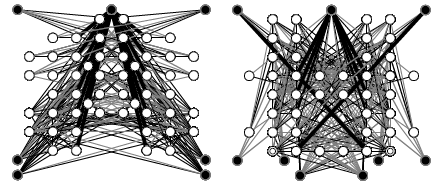
\includegraphics[scale=0.55]{images/hyperneatnets.png}
\caption{A CPPN at gen 30 (left) and gen 106 (right) evolved by HyperNEAT \cite{hyperpic}}
\end{figure}

\section{Deep Convolutional Networks}
Deep Convolutional Networks (DCNs) are another class of machine learning algorithms closely related to ANNs.  DCNs are a subset of feed-forward ANNs which contain a number of what are called \textit{convolutional} hidden layers, and are traditionally created for image recognition.  However, as seen in Google's Go playing machine AlphaGo \cite{alphago}, DCNs can be adapted for other tasks as well.

DCNs are far more complex than a simple feed-forward ANN, and to understand them it is perhaps best to think of each layer as a square of nodes rather than a line (Figure \ref{ref:dcn1}).  Each layer still only directly interacts with the very next layer, but each hidden node will only be connected to a small region or window of the input nodes.  This window then ``slides'' over the input layer for each hidden node, with overlap.  This concept is awkward to explain in words, but Figure \ref{ref:dcnmain} represents how this works graphically.

\begin{figure}[h]
\centering
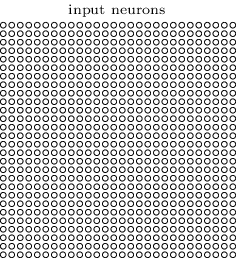
\includegraphics[scale=0.5]{images/dcn1.png}
\caption{DCN input layer \cite{handwriting}}
\label{ref:dcn1}
\end{figure}

This mapping of small windows of nodes onto a single node through several hidden layers is repeated over a number of layers.  After the convolutional layers, there are a series of \textit{pooling} or \textit{subsampling} layers.  These are similar to the convolutional layers in that they still link a region of nodes onto a node in the next layer, but in much smaller groups, perhaps 2x2.  The output of each pooling layer is usually either the maximum or the minimum value from its grid of inputs.  The goal of this process is to simplify the output of the convolutional layers.

\begin{figure*}[h!]
    \centering
    \begin{subfigure}[t]{0.5\textwidth}
        \centering
        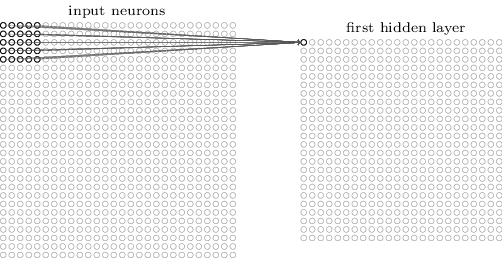
\includegraphics[height=1.4in]{images/dcnmain1.png}
        \caption{Links from input layer to hidden node 1}
    \end{subfigure}%
    ~ 
    \begin{subfigure}[t]{0.5\textwidth}
        \centering
        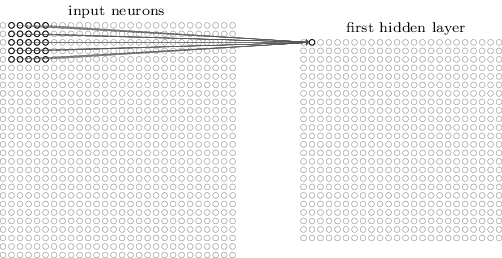
\includegraphics[height=1.4in]{images/dcnmain2.png}
        \caption{Links from input layer to hidden node 2}
    \end{subfigure}
    \caption{Links in a convolutional network\cite{handwriting}}
    \label{ref:dcnmain}
\end{figure*}

The pooling layers are linked with another layer of convolutional layers in the same way convolution was described before, and this back-and-forth between pooling and convolution is done how ever many times is wanted.  This process as a whole is called \textit{feature extraction}, because it allows the network to break a picture down into a representation of its most basic features.  After feature extraction, the final layers are connected to a standard, fully connected ANN which produces the output, usually a classification of the image.

\begin{figure}[h]
\centering
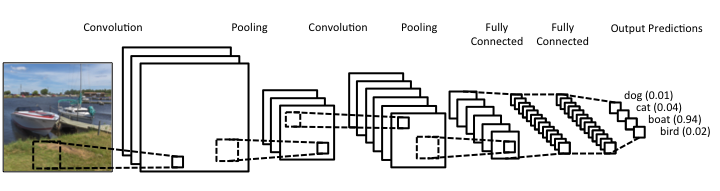
\includegraphics[scale=0.5]{images/cnnfull.png}
\caption{An example of a full DCN \cite{clarifai}}
\label{ref:cnnfull}
\end{figure}

Perhaps the most famous implementation of a DCN with MCTS is Google DeepMind's Alphago \cite{alphago}.  AlphaGo is designed by Google DeepMind which plays the board game Go, and in 2015, it became the first computer program to beat a professional human Go player without handicaps on a full board.  AlphaGo uses MCTS in conjunction with three different DCNs --- two are called ``policy networks'' and essentially alter the tree and default policy of MCTS, while the third is a ``value network'' and helps determine the value of the current game state.  Each network had 13 hidden layers.

AlphaGo was trained in two phases. First, the network was trained on millions of moves from professional Go games. This training was done until the program could predict a human move 57\% of the time. The second phase of training involved AlphaGo playing itself and, using reinforcement learning, discovering new strategies for itself. The result was an incredibly intelligent system --- AlphaGo was able to beat the next best Go AIs in 499 out of 500 games played, even when giving the other programs a four move headstart.\cite{alphago}